\documentclass{iitthesis}

\usepackage[utf8]{inputenc}
\usepackage[T1]{fontenc}

\usepackage{cite}
\usepackage{amsmath} % \boldsymbol
\usepackage{graphicx} % \includegraphics
\usepackage[nodayofweek]{datetime} % \today

% If we use hyperref, we can automatically embed this metadata into the PDF
\usepackage{hyperref}
\hypersetup{pdftex,
	hidelinks, % I don't like when it makes those colored boxes around hyperlinks, comment out to restore
	pdfauthor={Keith Pedersen (Keith.David.Pedersen@gmail.com)},
	pdftitle={Modified "iitthesis.cls" and helper scripts},
	pdfsubject={Making it slightly easier to compiler your thesis.},
	pdfkeywords={iitthesis.cls, IIT, thesis, Latex, list of figures}}
	
% Make sure that \includegraphics finds pdf BEFORE png (the default is png first)
% https://tex.stackexchange.com/questions/45498/choosing-whether-to-include-pdf-or-png-in-pdflatex
\usepackage{grfext}
\PrependGraphicsExtensions*{.pdf}

\begin{document}

\title{Modified ``{\tt iitthesis.cls}'' and helper scripts}

%~ \title{Bold math in section headings with}

%Thesis Proposal}
\author{Keith Pedersen}
\degree{Master of the Universe}
\dept{perpetuity}
\date{\today} % (NOT used in your thesis; it should say your graduating month and year only).

\signaturetrue
%\coadvisortrue           % add co-advisor. activate it by removing % symbol to add co-advisor
\maketitle

\prelimpages

\begin{acknowledgement}     % acknowledgement environment, this is optional

	This acknowledgment is here so the table of contents is numbered correctly.
\end{acknowledgement}

\tableofcontents
\clearpage

\listoffigures
\clearpage

\begin{abstract}
	
	This document describes the modifications I have made to the 
	{\tt iitthesis.cls} \LaTeX{} class file, with instructions for its use.
	Also included are several shell scripts and Python programs for 
	performing some ancillary tasks.
		
	{\bf NOTE:} My scripts ({\tt *.sh}) are written for a Bash shell environment 
	(as one finds on a GNU+Linux operating system).
	They were not designed to be simple, portable, or user friendly;
	they were written out of necessity under a terrible time crunch, 
	and I am supplying them to the public as a courtesy to my Physics colleagues.
	I have not used Windows in five years, and have never used Mac OS, 
	so please, \emph{please}, \emph{\textbf{please}} don't contact me 
	asking for help getting the scripts to work on Windows or Mac. 
	I don't know, have no inclination to learn, 
	and \emph{will not} attempt to help you. 
	I will also not provide general \LaTeX{} help.
	I know this is cold, but I am very busy.
	I expect that any PhD candidate trying to use \LaTeX{} is at least
	somewhat savvy with coding, so find out who else is graduating in your term and 
	form an {\tt iitthesis.cls} user group; hopefully you can help each other.
	Or look online; that's how I learned to do most of this stuff.
		
	I will, however, help correct bugs in my scripts and programs.
	If you find one, email a detailed log of the error to the email listed on my GitHub	
	(better yet, send me a minimum working example of your thesis folder
	zipped/tar'd into a single compressed file). 
	If you can fix the bug yourself, please \emph{let me know} so I can correct the repo
	(or submit a pull request to GitHub, so I can review/approve your edits).
\end{abstract}

\textpages

%%%%%%%%%%%%%%%%%%%%%%%%%%%%%%%%%%%%%%%%%%%%%%%%%%%%%%%%%%%%%%%%%%%%%%%%
%%%%%%%%%%%%%%%%%%%%%%%%%%%%%%%%%%%%%%%%%%%%%%%%%%%%%%%%%%%%%%%%%%%%%%%%
%%%%%%%%%%%%%%%%%%%%%%%%%%%%%%%%%%%%%%%%%%%%%%%%%%%%%%%%%%%%%%%%%%%%%%%%
%%%%%%%%%%%%%%%%%%%%%%%%%%%%%%%%%%%%%%%%%%%%%%%%%%%%%%%%%%%%%%%%%%%%%%%%

\Chapter{Compiling the modified {\tt iitthesis.cls}}

Lucky for you, this is the shortest chapter. 
On your computer, there is a director that 
contains your main \LaTeX{} file (e.g., {\tt myThesis.tex});
I will refer to this as your ``main directory''.
Clone the Git repo~\cite{Pedersen:iitthesis} into the main directory.
From that main directory, run the shell script {\tt iitthesis/makeLinks.sh}.
This will create a number of soft links and copy one file ({\tt MakeMyThesis.sh}).
Open {\tt MakeMyThesis.sh} and change the variable {\tt baseName}
to be the name of your main \LaTeX{} file, minus the {\tt .tex} extension 
(e.g., {\tt baseName=myThesis}).
Be careful not to add spaces; Bash doesn't like them.
Now compile your thesis by running {\tt MakeMyThesis.sh}.
To make the final version (and embed fonts),
pass {\tt MakeMyThesis.sh} a dummy argument (any value/string will do).



%%%%%%%%%%%%%%%%%%%%%%%%%%%%%%%%%%%%%%%%%%%%%%%%%%%%%%%%%%%%%%%%%%%%%%%%
%%%%%%%%%%%%%%%%%%%%%%%%%%%%%%%%%%%%%%%%%%%%%%%%%%%%%%%%%%%%%%%%%%%%%%%%
%%%%%%%%%%%%%%%%%%%%%%%%%%%%%%%%%%%%%%%%%%%%%%%%%%%%%%%%%%%%%%%%%%%%%%%%
%%%%%%%%%%%%%%%%%%%%%%%%%%%%%%%%%%%%%%%%%%%%%%%%%%%%%%%%%%%%%%%%%%%%%%%%

\Chapter{Your \LaTeX{} preamble}

%%%%%%%%%%%%%%%%%%%%%%%%%%%%%%%%%%%%%%%%%%%%%%%%%%%%%%%%%%%%%%%%%%%%%%%%
%%%%%%%%%%%%%%%%%%%%%%%%%%%%%%%%%%%%%%%%%%%%%%%%%%%%%%%%%%%%%%%%%%%%%%%%
%%%%%%%%%%%%%%%%%%%%%%%%%%%%%%%%%%%%%%%%%%%%%%%%%%%%%%%%%%%%%%%%%%%%%%%%

\Section{{\tt hyperref} to embed metadata}

It looks nice when your PDF file has metadata (a title, author, keywords, etc.). 
This can be easily and automatically inserted via the {\tt hyperref} package, 
using a \verb|\hypersetup| environment in your \LaTeX{} preamble.
For an example, look no further than the {\tt KDPmods.tex} file used to compile this document.
Note that I disable the colored boxes around hyperlinks,
because I find them distracting to the eye. 
Disabling the boxes does not disable the clickability of the links themselves

%%%%%%%%%%%%%%%%%%%%%%%%%%%%%%%%%%%%%%%%%%%%%%%%%%%%%%%%%%%%%%%%%%%%%%%%
%%%%%%%%%%%%%%%%%%%%%%%%%%%%%%%%%%%%%%%%%%%%%%%%%%%%%%%%%%%%%%%%%%%%%%%%
%%%%%%%%%%%%%%%%%%%%%%%%%%%%%%%%%%%%%%%%%%%%%%%%%%%%%%%%%%%%%%%%%%%%%%%%

\Section{Your advisor signature}

A major pain in the ass is embedding your advisor's signature into your final PDF, 
for submission to the thesis website. My advisor showed me a way to 
stitch PDFs together using the {\tt pdftk} program, but not only is it a pain, 
it also strips any metadata inserted using {\tt hyperref}.
I found a much better way by modifying the {\tt iitthesis.cls} file directly.

Follow these steps to use my modification:
\begin{enumerate}
	\item Print the first page of your thesis using \verb|\signaturefalse|
	(which should appear before the \verb|\maketitle| command).
	This should obtain the blank Advisor signature line in the original {\tt iitthesis.cls}.
	
	\item Have your advisor sign the page. Their signature \emph{must not} extend
	past the right edge of the signature line, 
	otherwise the horizontal alignment will be off.
	
	\item Scan the signature into a high-resolution image. 
	Preserving the original dimensions of the scan,
	crop the image (adding a thin white margin) so that:
	%
	\begin{enumerate}
	
		\item ``Approved'' is at the image's left edge.
		
		\item ``Advisor'' is at the image's bottom edge.
		
		\item The black line ends at image's right edge.
		
		\item The highest point of the signature is at the image's top edge.
		
	\end{enumerate}
	%	
	See ``./Figures/ZackSignature.pdf'' for an example.
	
	Thank me for this, but it actually doesn't matter how tall the signature is.
	I have written the modification to \emph{automatically adjust} 
	the vertical alignment to account for the height of the signature.	
	
	\item Name the signature image "AdvisorSignature.xxx" 
	(replacing xxx with the appropriate format extension, 
	although you are limited to image formats supported by \verb|\includegraphics|)
	and place in the same directory as your main {\tt .tex} file.
	I created a link instead of renaming the image; this works too.
	
	\item Change the preamble to \verb|\signaturetrue|.
	The signed line should now appear in roughly the same location 
	as the blank line (toggle \verb|\signaturefalse| to verify).
	
\end{enumerate}
%
Unfortunately, there is currently no support for the co-advisor signature.
But hopefully, someone will need this feature and, 
following my example in {\tt iitthesis.cls} (search for KDP), will add the proper code.

%%%%%%%%%%%%%%%%%%%%%%%%%%%%%%%%%%%%%%%%%%%%%%%%%%%%%%%%%%%%%%%%%%%%%%%%
%%%%%%%%%%%%%%%%%%%%%%%%%%%%%%%%%%%%%%%%%%%%%%%%%%%%%%%%%%%%%%%%%%%%%%%%
%%%%%%%%%%%%%%%%%%%%%%%%%%%%%%%%%%%%%%%%%%%%%%%%%%%%%%%%%%%%%%%%%%%%%%%%
%%%%%%%%%%%%%%%%%%%%%%%%%%%%%%%%%%%%%%%%%%%%%%%%%%%%%%%%%%%%%%%%%%%%%%%%

\Chapter{Section and subsection titles (and removing bold math from the table of contents)}

%%%%%%%%%%%%%%%%%%%%%%%%%%%%%%%%%%%%%%%%%%%%%%%%%%%%%%%%%%%%%%%%%%%%%%%%
%%%%%%%%%%%%%%%%%%%%%%%%%%%%%%%%%%%%%%%%%%%%%%%%%%%%%%%%%%%%%%%%%%%%%%%%
%%%%%%%%%%%%%%%%%%%%%%%%%%%%%%%%%%%%%%%%%%%%%%%%%%%%%%%%%%%%%%%%%%%%%%%%

\Section{A section about $\sqrt{x^2+y^2}$}\label{sec:no-bold-in-text}

This section is about math (at least it claims to be).
But notice how the math is not bolded in the section title?
This is because \verb|\textbf| is automatically wrapped around the section title,
but \verb|\textbf| does not alter the math environment \verb|$\sqrt{x^2+y^2}$|.

%%%%%%%%%%%%%%%%%%%%%%%%%%%%%%%%%%%%%%%%%%%%%%%%%%%%%%%%%%%%%%%%%%%%%%%%
%%%%%%%%%%%%%%%%%%%%%%%%%%%%%%%%%%%%%%%%%%%%%%%%%%%%%%%%%%%%%%%%%%%%%%%%
%%%%%%%%%%%%%%%%%%%%%%%%%%%%%%%%%%%%%%%%%%%%%%%%%%%%%%%%%%%%%%%%%%%%%%%%

\Section{A section about $\boldsymbol{\sqrt{1-x^2}}$ (bolded in the heading)}\label{sec:bold-in-TOC}

I can bold the math in this section title by using the {\tt amsmath} package 
(i.e.\ \verb|\usepackage{amsmath}|), and wrapping {\tt \verb|\boldsymbol|} around my math

	\verb|\Section{A section about $\boldsymbol{\sqrt{x^2+y^2}}$}|

\noindent 
However, this bold math will also appear in the (TOC), 
which is not supposed to be bolded.
There is no way to instruct {\tt iitthesis.cls} to use \verb|\boldmath|
for the main heading, but not for the TOC (at least not without me learning some deep TeX, 
the much less user friendly markup language that \LaTeX{} is based upon).

Luckily I was able to find a hack. It relies on understanding how the TOC works.
Each call to {\tt pdflatex} generates a {\tt .toc} file, 
which lists everything that should show up in the TOC. 
This file is used \emph{the next} time that {\tt pdflatex} is called. 
There are several such intermediate files created ({\tt .toc}, {\tt .bbl}, {\tt .lof}, etc),
and each is not actually used until the next call to {\tt pdflatex}
(this is why it often takes three calls to {\tt pdflatex} before all 
the citations work correctly).

To fix this problem, I wrote a Python program to scan the {\tt .toc} file 
after each call to {\tt pdflatex} and removes all \verb|\boldmath|.
Luckily, you don't have to use this program directly; 
all you have to do is run the Bash script {\tt MakeMyThesis.sh}.

%%%%%%%%%%%%%%%%%%%%%%%%%%%%%%%%%%%%%%%%%%%%%%%%%%%%%%%%%%%%%%%%%%%%%%%%
%%%%%%%%%%%%%%%%%%%%%%%%%%%%%%%%%%%%%%%%%%%%%%%%%%%%%%%%%%%%%%%%%%%%%%%%
%%%%%%%%%%%%%%%%%%%%%%%%%%%%%%%%%%%%%%%%%%%%%%%%%%%%%%%%%%%%%%%%%%%%%%%%

\Section{Optional punctuation arguments for subsections and subsubsections}

Subsection titles have punctuation automatically appended to their title. 
They are also not supposed to have any space after the title
(so make sure you comment out any blank lines, see {\tt KDPmods.tex}).

%%%%%%%%%%%%%%%%%%%%%%%%%%%%%%%%%%%%%%%%%%%%%%%%%%%%%%%%%%%%%%%%%%%%%%%%
%%%%%%%%%%%%%%%%%%%%%%%%%%%%%%%%%%%%%%%%%%%%%%%%%%%%%%%%%%%%%%%%%%%%%%%%

\Subsection{The automatic period}
% 
The default punctuation for sections (and subsubsection) is the period.

%%%%%%%%%%%%%%%%%%%%%%%%%%%%%%%%%%%%%%%%%%%%%%%%%%%%%%%%%%%%%%%%%%%%%%%%

\Subsubsection{Don't pass your own period.}
% 
If you pass a period, you will get two.

\begin{verb}
	\Subsubsection{Don't pass your own period.}
\end{verb}

%%%%%%%%%%%%%%%%%%%%%%%%%%%%%%%%%%%%%%%%%%%%%%%%%%%%%%%%%%%%%%%%%%%%%%%%
%%%%%%%%%%%%%%%%%%%%%%%%%%%%%%%%%%%%%%%%%%%%%%%%%%%%%%%%%%%%%%%%%%%%%%%%

\Subsection[?]{Do all subsections have to end in a period}
%
No! With my modification to {\tt iitthesis.cls}, an optional argument can be passed to send
some other punctuation. This optional argument defaults to a period
(i.e.\ if you want a period, you don't have to pass it).

\begin{verb}
	\Subsection[?]{Do all subsections have to end in a period}
\end{verb}

%%%%%%%%%%%%%%%%%%%%%%%%%%%%%%%%%%%%%%%%%%%%%%%%%%%%%%%%%%%%%%%%%%%%%%%%

\Subsubsection[!]{It also work for subsubsections} Huzzah!

%%%%%%%%%%%%%%%%%%%%%%%%%%%%%%%%%%%%%%%%%%%%%%%%%%%%%%%%%%%%%%%%%%%%%%%%

\Subsubsection[~:(]{Be careful}
% 
You can pass any string as punctuation, but not all are acceptable.
 
\begin{verb}
	\Subsubsection[~:(]{Be careful}
\end{verb}

%%%%%%%%%%%%%%%%%%%%%%%%%%%%%%%%%%%%%%%%%%%%%%%%%%%%%%%%%%%%%%%%%%%%%%%%
%%%%%%%%%%%%%%%%%%%%%%%%%%%%%%%%%%%%%%%%%%%%%%%%%%%%%%%%%%%%%%%%%%%%%%%%
%%%%%%%%%%%%%%%%%%%%%%%%%%%%%%%%%%%%%%%%%%%%%%%%%%%%%%%%%%%%%%%%%%%%%%%%
%%%%%%%%%%%%%%%%%%%%%%%%%%%%%%%%%%%%%%%%%%%%%%%%%%%%%%%%%%%%%%%%%%%%%%%%

\Chapter{Remove citations from the list of figures}

\begin{figure}[h]
\centering
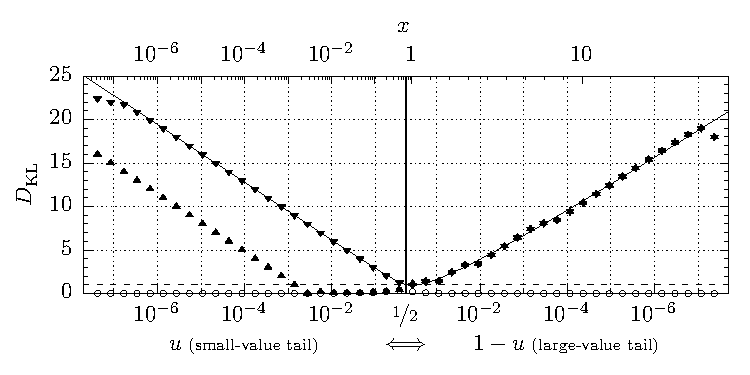
\includegraphics[scale=1]{Figures/infoLoss_exponential.pdf}
\caption{My favorite figure from my thesis~\cite{Pedersen:thesis}.}
\label{fig:favorite}
\end{figure}

If you cite a figure in its caption (i.e., you include someone else's figure for reference), 
then by default that citation will appear in the list of figures.
This is unfortunate, because \LaTeX{} will automatically number
citations by the order they appear in the document.
This means that any citation which appears in a figure caption
will be numbered before any citation in the body of your thesis, 
even if the figure doesn't appear until page 137
(i.e., citations 1--15 are all the citations appearing in figure captions).

The best way to fix this would be for the list of figures to use 
short captions (condensed main captions). These can be passed as 
optional arguments before the main caption:

\begin{verb}
	\caption[Short caption]{A much longer, more detailed caption}
\end{verb}

\noindent
The long, detailed caption will appear below the figure, 
and the short caption in the list of figures. 
Unfortunately, the IIT style guide \emph{requires} the list of figures to contain
\emph{the exact same} caption as below the figure.

Thus, I have created another Python program to strip captions from the 
list of figures file ({\tt .lof}). Notice how Figure~\ref{fig:favorite}
cites my thesis, but the citation does not appear in the list of figures?
You won't get this without running my program. However, 
just like the program that strips the bold math from the table of contents,
you don't have to use it directly; it will run automatically in {\tt MakeMyThesis.sh}.

%%%%%%%%%%%%%%%%%%%%%%%%%%%%%%%%%%%%%%%%%%%%%%%%%%%%%%%%%%%%%%%%%%%%%%%%
%%%%%%%%%%%%%%%%%%%%%%%%%%%%%%%%%%%%%%%%%%%%%%%%%%%%%%%%%%%%%%%%%%%%%%%%
%%%%%%%%%%%%%%%%%%%%%%%%%%%%%%%%%%%%%%%%%%%%%%%%%%%%%%%%%%%%%%%%%%%%%%%%
%%%%%%%%%%%%%%%%%%%%%%%%%%%%%%%%%%%%%%%%%%%%%%%%%%%%%%%%%%%%%%%%%%%%%%%%

\Chapter{Embedding fonts from PDF figures}

Your thesis will compile much quicker (and look much better) if you use PDF figures.
This is because PDFs are containers, and the contents of figure PDFs
are literally injected into the thesis unaltered. 
This requires no rendering and preserves the resolution of the figure. 
I always use PDF figures (with vector graphics under the hood)
because they render perfectly at any screen resolution
(especially if you are giving a presentation about your work on a big screen).\footnote
{\nobreak % This prevents an extra space between footnote number and words if the words begin on the line after the open brace
	I prefer not to supply the file extension when I include a figure
	(for whatever reason).
	%
	% No verbatim code in a footnote
	% \begin{verb}
	%    \includegraphics[scale=1]{Figures/myFig}
	% \end{verb}
	%
	% \noindent
	But by default, {\tt graphicx} will search for a PNG before a PDF! 
	So if you have two versions of a figure
	--- a PDF for your thesis and a PNG for PowerPoint or your website ---
	then {\tt graphicx} will choose the down-sampled PNG for insertion into your thesis. 
	Making PDF come first requires a two-line fix in the preamble 
	(search for {\tt grfext} in {\tt KDPmods.tex}).
}

Unfortunately, not all programs that export PDFs embed the fonts by default. 
Not embedding saves space (simply reference the font by name, 
then look it up on the system that's viewing the PDF),
but it is a really bad idea because not every system has every font (especially funny math fonts).
Ever seen a presentation where one slide's math was broken, 
or some part of a figure was missing? They probably didn't embed their fonts, 
and one font didn't exist on the laptop being used to run the projector.
Fonts don't take a lot of space, so for maximum portability, 
they should be embedded in every PDF.
I generally use {\tt gnuplot} to make my figures, which always embeds its fonts
(to check for embedding, run {\tt pdffonts} and look for a ``yes'' in the ``emb'' column).

But there are still two problems:
(i) if you are borrowing figures from another paper (citing it, of course), 
\emph{that author} may not have embedded their fonts and 
(ii) if 70 figures all use font XYZ, and XYZ is embedded in each PDF,
then XYZ will be embedded in the main thesis PDF 70 times 
(since PDF figures are simply injected as-is, embedded fonts and all).
To fix these problems, we'd like to embed any fonts that aren't embedded, 
while also ensuring that each unique font is only embedded once.
This is what the script {\tt fontembed.sh} does.
It takes a bit of time to run, but it will make your PDF much more portable
(and potentially much smaller; my thesis shrinks by 33\% when I consolidate fonts).

Luckily, just like the Python programs that fix the table of contents and list of figures, 
{\tt fontembed.sh} is run automatically by {\tt MakeMyThesis.sh}.
However, it does require that you have GhostScript installed on your system. 
Furthermore, it takes a significant amount of time to run, 
so {\tt MakeMyThesis.sh} only embeds fonts when you pass the extra dummy argument. 
The dummy argument tells the script to create a final version of your thesis
with a different name (e.g., myThesis\_Final.pdf).
This final version is the one with the embedded fonts
(a version without embedded fonts is also retained, using the normal name).

\bibliographystyle{unsrt} % Dr. Pat approved this style for my thesis
\bibliography{KDPmods}

\end{document}
